\documentclass[xcolor={dvipsnames}]{beamer}
%\usepackage[utf8]{inputenc}
\usetheme{Madrid}
%\usetheme{Malmoe}
\usecolortheme{beaver}
%\usecolortheme{rose}

%-------------------------------------------------------------------------------
%          -Packages nécessaires pour écrire en Français et en UTF8-
%-------------------------------------------------------------------------------
\usepackage[utf8]{inputenc}
\usepackage[frenchb]{babel}
\usepackage[T1]{fontenc}
\usepackage{lmodern}
\usepackage{textcomp}

%-------------------------------------------------------------------------------

%-------------------------------------------------------------------------------
%                          -Outils de mise en forme-
%-------------------------------------------------------------------------------
\usepackage{hyperref}
\hypersetup{pdfstartview=XYZ}
\usepackage{enumerate}
\usepackage{graphicx}
%\usepackage{multicol}
%\usepackage{tabularx}

%\usepackage{anysize} %%pour pouvoir mettre les marges qu'on veut
%\marginsize{2.5cm}{2.5cm}{2.5cm}{2.5cm}

\usepackage{indentfirst} %%pour que les premier paragraphes soient aussi indentés
\usepackage{verbatim}
%\usepackage[table]{xcolor}  
%\usepackage{multirow}
\usepackage{ulem}
%-------------------------------------------------------------------------------


%-------------------------------------------------------------------------------
%                  -Nécessaires pour écrire des mathématiques-
%-------------------------------------------------------------------------------
\usepackage{amsfonts}
\usepackage{amssymb}
\usepackage{amsmath}
\usepackage{amsthm}
\usepackage{tikz}
\usepackage{xlop}
\usepackage[output-decimal-marker={,}]{siunitx}
%-------------------------------------------------------------------------------


%-------------------------------------------------------------------------------
%                    - Mise en forme 
%-------------------------------------------------------------------------------

\newcommand{\bu}[1]{\underline{\textbf{#1}}}


\usepackage{ifthen}


\newcommand{\ifTrue}[2]{\ifthenelse{\equal{#1}{true}}{#2}{$\qquad \qquad$}}

\newcommand{\kword}[1]{\textcolor{red}{\underline{#1}}}


%-------------------------------------------------------------------------------



%-------------------------------------------------------------------------------
%                    - Racourcis d'écriture -
%-------------------------------------------------------------------------------

% Angles orientés (couples de vecteurs)
\newcommand{\aopp}[2]{(\vec{#1}, \vec{#2})} %Les deuc vecteurs sont positifs
\newcommand{\aopn}[2]{(\vec{#1}, -\vec{#2})} %Le second vecteur est négatif
\newcommand{\aonp}[2]{(-\vec{#1}, \vec{#2})} %Le premier vecteur est négatif
\newcommand{\aonn}[2]{(-\vec{#1}, -\vec{#2})} %Les deux vecteurs sont négatifs

%Ensembles mathématiques
\newcommand{\naturels}{\mathbb{N}} %Nombres naturels
\newcommand{\relatifs}{\mathbb{Z}} %Nombres relatifs
\newcommand{\rationnels}{\mathbb{Q}} %Nombres rationnels
\newcommand{\reels}{\mathbb{R}} %Nombres réels
\newcommand{\complexes}{\mathbb{C}} %Nombres complexes


%Intégration des parenthèses aux cosinus
\newcommand{\cosP}[1]{\cos\left(#1\right)}
\newcommand{\sinP}[1]{\sin\left(#1\right)}

%Fractions
\newcommand{\myfrac}[2]{{\LARGE $\frac{#1}{#2}$}}

%Vocabulaire courrant
\newcommand{\cad}{c'est-à-dire}

%Droites
\newcommand{\dte}[1]{droite $(#1)$}
\newcommand{\fig}[1]{figure $#1$}
\newcommand{\sym}{symétrique}
\newcommand{\syms}{symétriques}
\newcommand{\asym}{axe de symétrie}
\newcommand{\asyms}{axes de symétrie}
\newcommand{\seg}[1]{$[#1]$}
\newcommand{\monAngle}[1]{$\widehat{#1}$}
\newcommand{\bissec}{bissectrice}
\newcommand{\mediat}{médiatrice}
\newcommand{\ddte}[1]{$[#1)$}

%Figures
\newcommand{\para}{parallélogramme}
\newcommand{\paras}{parallélogrammes}
\newcommand{\myquad}{quadrilatère}
\newcommand{\myquads}{quadrilatères}
\newcommand{\co}{côtés opposés}
\newcommand{\diag}{diagonale}
\newcommand{\diags}{diagonales}
\newcommand{\supp}{supplémentaires}
\newcommand{\car}{carré}
\newcommand{\cars}{carrés}
\newcommand{\rect}{rectangle}
\newcommand{\rects}{rectangles}
\newcommand{\los}{losange}
\newcommand{\loss}{losanges}


%----------------------------------------------------


\usepackage{../../../../pas-math}
\usepackage{../../../../moncours_beamer}

\usepackage{amssymb,amsmath}


\newcommand{\myitem}{\item[\textbullet]}

\graphicspath{{../img/}}

\title{Séquence 2 : Droites, segments et codage}
%\author{O. FINOT}\institute{Collège S$^t$ Bernard}

%
\AtBeginSection[]
{
	\begin{frame}
		\frametitle{}
		\tableofcontents[currentsection, hideallsubsections]
	\end{frame} 

}
%
%
%\AtBeginSubsection[]
%{
%	\begin{frame}
%		\frametitle{Sommaire}
%		\tableofcontents[currentsection, currentsubsection]
%	\end{frame} 
%}

\begin{document}



\begin{frame}
  \titlepage 
\end{frame}


\begin{frame}{}
	\begin{myobj}
	\begin{itemize}
		
		\item Construire le symétrique d’un point ou d'une figure par rapport à une droite à la main où à l’aide d’un logiciel;
		\item Construire le symétrique d’un point ou d'une figure par rapport à un point, à la main où à l’aide d’un logiciel;
		\item Utiliser les propriétés de la symétrie axiale ou centrale;
		\item Identifier des symétries dans des figures.		
	\end{itemize}
\end{myobj}

\begin{mycomp}
	\begin{itemize}
		\item \kw{Chercher (Ch2)} :  s’engager    dans    une    démarche    scientifique, observer, questionner, manipuler, expérimenter (sur une feuille de papier, avec des objets, à l’aide de logiciels), émettre des hypothèses, chercher des exemples ou des contre-exemples, simplifier ou particulariser une situation, émettre une conjecture ;
		\item \kw{Raisonner (Ra3)} :  démontrer : utiliser un raisonnement logique et des règles établies (propriétés, théorèmes, formules) pour parvenir à une conclusion ;
		\item \kw{Communiquer (Co2)} :  expliquer à l’oral ou à l’écrit (sa démarche, son raisonnement, un calcul, un protocole   de   construction   géométrique, un algorithme), comprendre les explications d’un autre et argumenter dans l’échange ; 
		
	\end{itemize}
\end{mycomp}



\end{frame}

\section{Droites}




\begin{frame}{}

	\begin{mydef}
		Une \kword{droite} est un objet géométrique formé de \kword{points alignés}. Une droite est illimitée des deux cotés.\pause
	\end{mydef}
	
	\begin{myprops}
		\begin{itemize}
			\item Une droite qui passe par deux points $A$ et $B$, se note $(AB)$ ou $(BA)$;
			\item Si un point $C$ appartient à la droite $(AB)$, on note $C \in (AB)$.
			\item Si il n'appartient pas à la droite $(AB)$, on note $C \notin (AB)$.\pause
		\end{itemize}
	\end{myprops}
	
	\begin{myex}
		Les points $M$, $R$ et $A$ sont alignés.
		\begin{center}
			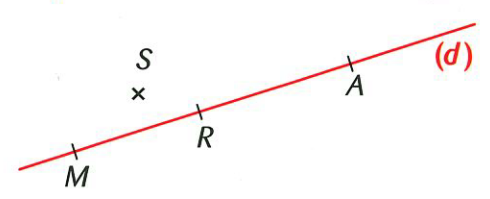
\includegraphics[scale=0.15]{../img/droite1}
		\end{center}
		
		\begin{itemize}
			\item La droite $(d)$ passant par les points $M$ et $R$ se note 
			\item Le point A appartient à la droite $(MR)$, on note :
			\item Le point S n'appartient pas à la droite $(MR)$, on note :
		\end{itemize}
	\end{myex}
\end{frame}

\begin{frame}
	\begin{mydef}
		Une \kword{demi-droite} est une portion de droite limitée d'un seul côté par un point, son \kword{origine}.\pause
	\end{mydef}
	
	\begin{myprop}
		La demi-droite d'origine $A$ et passant par $B$ se note $[AB)$.\pause
	\end{myprop}
	
	\begin{myex}
		\begin{center}
			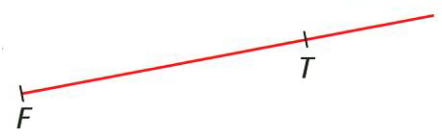
\includegraphics[scale=0.55]{../img/demi-droite}
		\end{center}
		
		La demi droite 
	\end{myex}
\end{frame}

\begin{frame}
	\begin{mydef}
		Un \kword{segment} est une portion de droite limitée par deux points : ses \kword{extrémités}.
	\end{mydef}
	
	
	\begin{myprop}
		Le segment d'extrémités $A$ et $B$ se note $[AB]$ ou $[BA]$.
	\end{myprop}
	
	\begin{myex}
		\begin{center}
			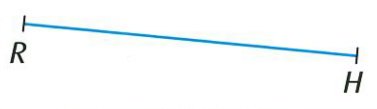
\includegraphics[scale=0.55]{../img/segment}
		\end{center}
		
		Le segment 
	\end{myex}
\end{frame}

\section{Longueurs et codages}


\begin{frame}
	\begin{mydef}
		La mesure (distance entre ses deux extrémités) d'un segment est sa \kword{longueur}.
	\end{mydef}
	
	\begin{myprop}
		La longueur d'un segment $[AB]$, se note $AB$ ou $BA$. 
	\end{myprop}
	
	\begin{myex}
		
		\begin{center}
			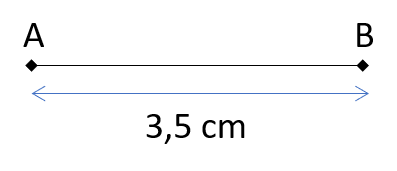
\includegraphics[scale=0.6]{../img/lgr}
		\end{center}
		
		La longueur du segment $[AB]$ est de \num{3.5} cm, on note
	\end{myex}
\end{frame}


\begin{frame}
	\begin{mydef}
		Le \kword{milieu} d'un segment est le point qui appartient au segment \kword{et} qui est à égale distance de ses extrémités.
	\end{mydef}
	
	\begin{myrem}
		Des segments de même longueur sont codés de façon identique.
	\end{myrem}
	
	\begin{myex}
		\begin{center}
			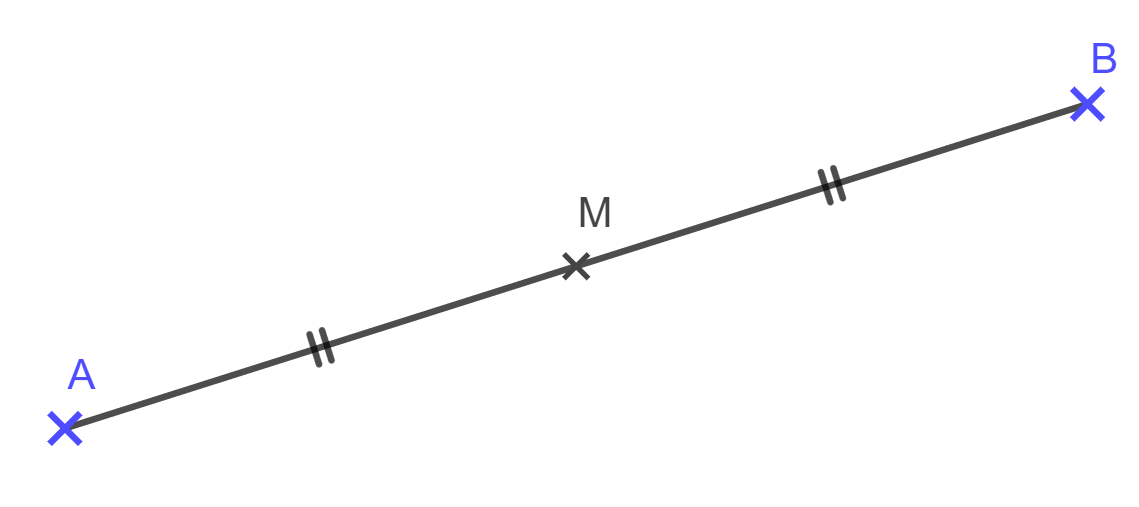
\includegraphics[scale=0.2]{../img/milieu}
		\end{center}
		
		On a : $M \in [AB]$ et $AM = MB$, donc le point $M$ est le milieu du segment $[AB]$. On a ainsi $AM = AB \div 2$. 
	\end{myex}
\end{frame}
\end{document}